\subsubsection{Arten von Software, inklusive SaaS}
Masse vs. individuell

\begin{itemize}
  \item \textbf{Standardsoftware} (packaged software) $\rightarrow$ allgemeingültig, häufig wiederkehrende Aufgabenstellung
  \item \textbf{Individualsoftware} (custom software) $\rightarrow$ ein Anwendungsfall, konkretes Aufgabenprofil
\end{itemize}

Kommerziell vs. open source

\begin{itemize}
  \item \textbf{kommerzielle Software} $\rightarrow$ Ziel: mit Verkauf und Nutzung Geld generieren, ohne Anpassung nutzbar (commercial of the shelf, cots)
  \item \textbf{Open-Source-Software} $\rightarrow$ Quelltext frei einsehbar, verschiedene Linzenzen (Freiheitsgrade) zur Nutzung und Verbreitung
\end{itemize}

Software-as-a-Service (SaaS)

\begin{itemize}
  \item \textbf{Softwaredistributionsmodell} $\rightarrow$ Dienstbezieher erhält Nutzungsrechte, Software wird bei Dienstleister betrieben, \textit{service level agreement} legt fest welche Folgen eine Unterschreitung der Dienstgüte hat (Ausfall, etc.)
\end{itemize}

\subsubsection{Tätigkeiten in Systementwicklung und -wartung}
6 große Themenbereiche

\begin{itemize}
  \item Geschäftsprozessmodellierung
  \item Requirements Engineering
  \item Entwurf
  \item Implementierung
  \item Softwaretest
  \item Change-Management
\end{itemize}

in den Phasen der IS-Systementwicklung

\begin{itemize}
  \item \textbf{Konzeptionsphase} $\rightarrow$ Management initiiert Projektmanagement/Anschaffungen, Entwicklung beginnt mit Geschäftsprozessmodellierung, Requirements Engineering
  \item \textbf{Umsetzungsphase} $\rightarrow$ Management zuständig für Steuerung/Konfigurationsmanagement, Entwicklung: vom Entwurf über Implementierung zu Tests
  \item \textbf{Einführungsphase} $\rightarrow$ Management weiter Konfigurationsmanagement und abschließendes PM, Entwicklung: Change-Management und Tests
  \end{itemize}
  
Grafisch dargestellt:

\begin{figure}[h]
\centering
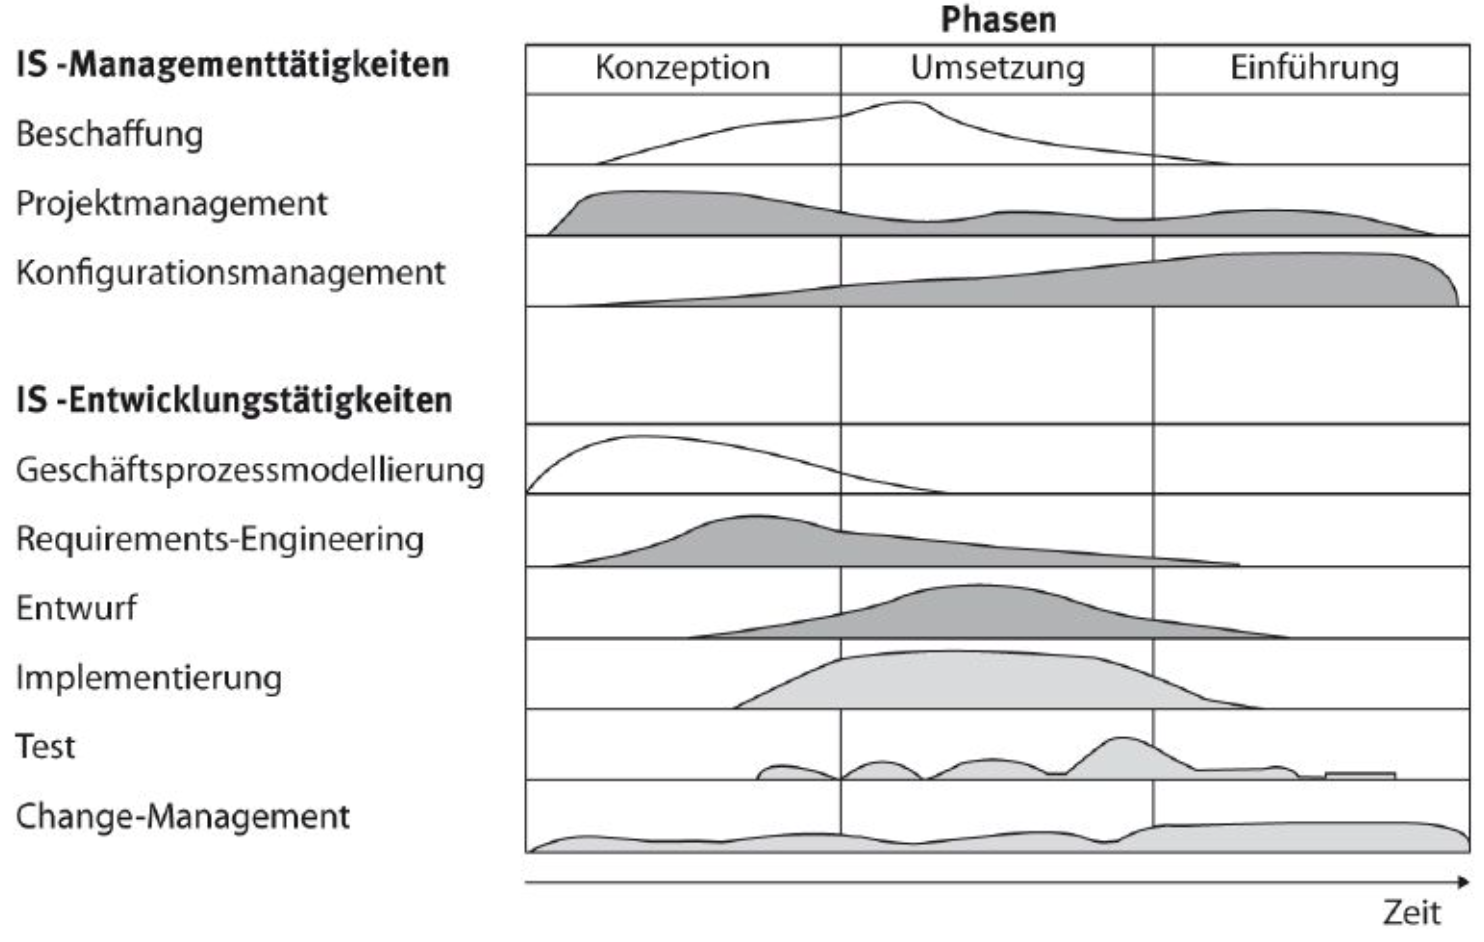
\includegraphics[width=0.8\textwidth]{assets/Phasen_Systementwicklung.png}
\end{figure}

\subsubsection{Requirements Engineering}
Definition

\begin{itemize}
  \item vollständige Gewinnung und Aufzeichnung der Anforderungen an ein System
  \item darauf aufbauend wird Anforderungsspezifikation erstellt
  \item daher möglichst vollständig, fehler- und widerspruchsfrei
\end{itemize}

Kategorie und Modellierung

\begin{itemize}
  \item \textbf{Kategorien} $\rightarrow$ funktionale vs. Qualitätsanforderungen
  \item \textbf{Anforderungsmodellierung} $\rightarrow$ abstrakte Zielmodelle, Szenarien (betrifft Benutzer z.B. BPMN), Lösungsmodelle (betrifft Entwickler z.B. ER)
\end{itemize}

Aufteilung in drei Aspekte

\begin{itemize}
  \item \textbf{Spezifikation} $\rightarrow$ korrekte Abbildung der Anforderungen (laufender Prozess)
  \item \textbf{Repräsentation} $\rightarrow$ Abbildung durch formale und informelle Beschreibungsmittel
  \item \textbf{Verhandlung} $\rightarrow$ unterschiedliche Interessen und Grade der Übereinstimmung mit Systemspezifikation sollen zu einer für alle Beteiligten akzeptierten und verständlichen Systemspezifikation werden
\end{itemize}

\subsubsection{Versionen von Software}
\begin{itemize}
  \item \textbf{Prototyp} $\rightarrow$ demonstrierbare Vorabversion zur Validierung eines Konzepts
  \item \textbf{Alphaversion} $\rightarrow$ nicht alle wesentlichen Funktionen enthalten, weitergebbar
  \item \textbf{Betaversion} $\rightarrow$ alle wesentlichen Funktionen enthalten, nicht vollständig getestet
  \item \textbf{Freigabekandidatenversion} $\rightarrow$ alle Funktionen vorhanden, vollständig getestet, größerer Test
  \item \textbf{Freigabeversion} $\rightarrow$ finale Version die an Dritte weitergegeben wird: Release
\end{itemize}

\subsubsection{Modelle: V-Modell XT, Scrum}
%Evtl Links in VL angucken
V-Modell XT: Überblick

\begin{itemize}
  \item entwickelt für Großprojekte im öffentlichen Bereich (Standard)
  \item regelt umfassend Detailschritte und Koordination zwischen Teilschritten, gut dokumentiert, Leitfaden
  \item interne und externe IS-Entwicklungsprojekte oder IS-Einführungsprojekte mit und ohne Softwareentwicklung
  \item Anpassung an konkretes Projekt erforderlich (XT $\rightarrow$ eXtreme tailoring)
\end{itemize}

V-Modell XT: Grundlagen

\begin{itemize}
  \item \textbf{Tailoring} $\rightarrow$ Zuschnitt auf konkretes Projekt zu Projektbeginn
  \item \textbf{Projekttypen} $\rightarrow$ Klassifizierung innerhalb des V-Modells und der Rollen, die die verschiedenen Parteien einnehmen
  \item \textbf{Produkttypvarianten} $\rightarrow$ Rahmenbedingungen für den Ablauf des Projekts (AG- oder AN-Projekt, Anzahl AN, neues Produkt vs. Pflege)
  \item \textbf{Produkte und Altivitäten} $\rightarrow$ Ergebnisse und Zwischenerebnisse werden als Produkt bezeichnet, die von Mitarbeitern mit definierten Rollen durch festgelegte Aktivitäten erzeugt werden, Produkt kann verschiedene Themen haben (dafür Aktivitäten)
  \item \textbf{Vorgehensbausteine} $\rightarrow$ zur Planung definiert, kapseln Aktivitäten, Produkte und Rollen
  \item \textbf{Projektdurchführungsstrategien} $\rightarrow$ wird durch Projektvariante und Projektmerkmale bestimmt, nicht durch Vorgehensbausteine
  \item \textbf{Entscheidungspunkte} $\rightarrow$ Meilenstein, Entscheidung über Fortführung und Freigabe der nächsten Phase
\end{itemize}

\clearpage
Agile Entwicklungsmodelle: Scrum

\begin{itemize}
  \item leichtgewichtig, unbürokratisch, kleine Teilprojektschritte mit greifbaren Ergebnissen und anpassbaren Vorgaben
  \item Teamwork, Selbstorganisation
\end{itemize}

\begin{figure}[h]
\centering
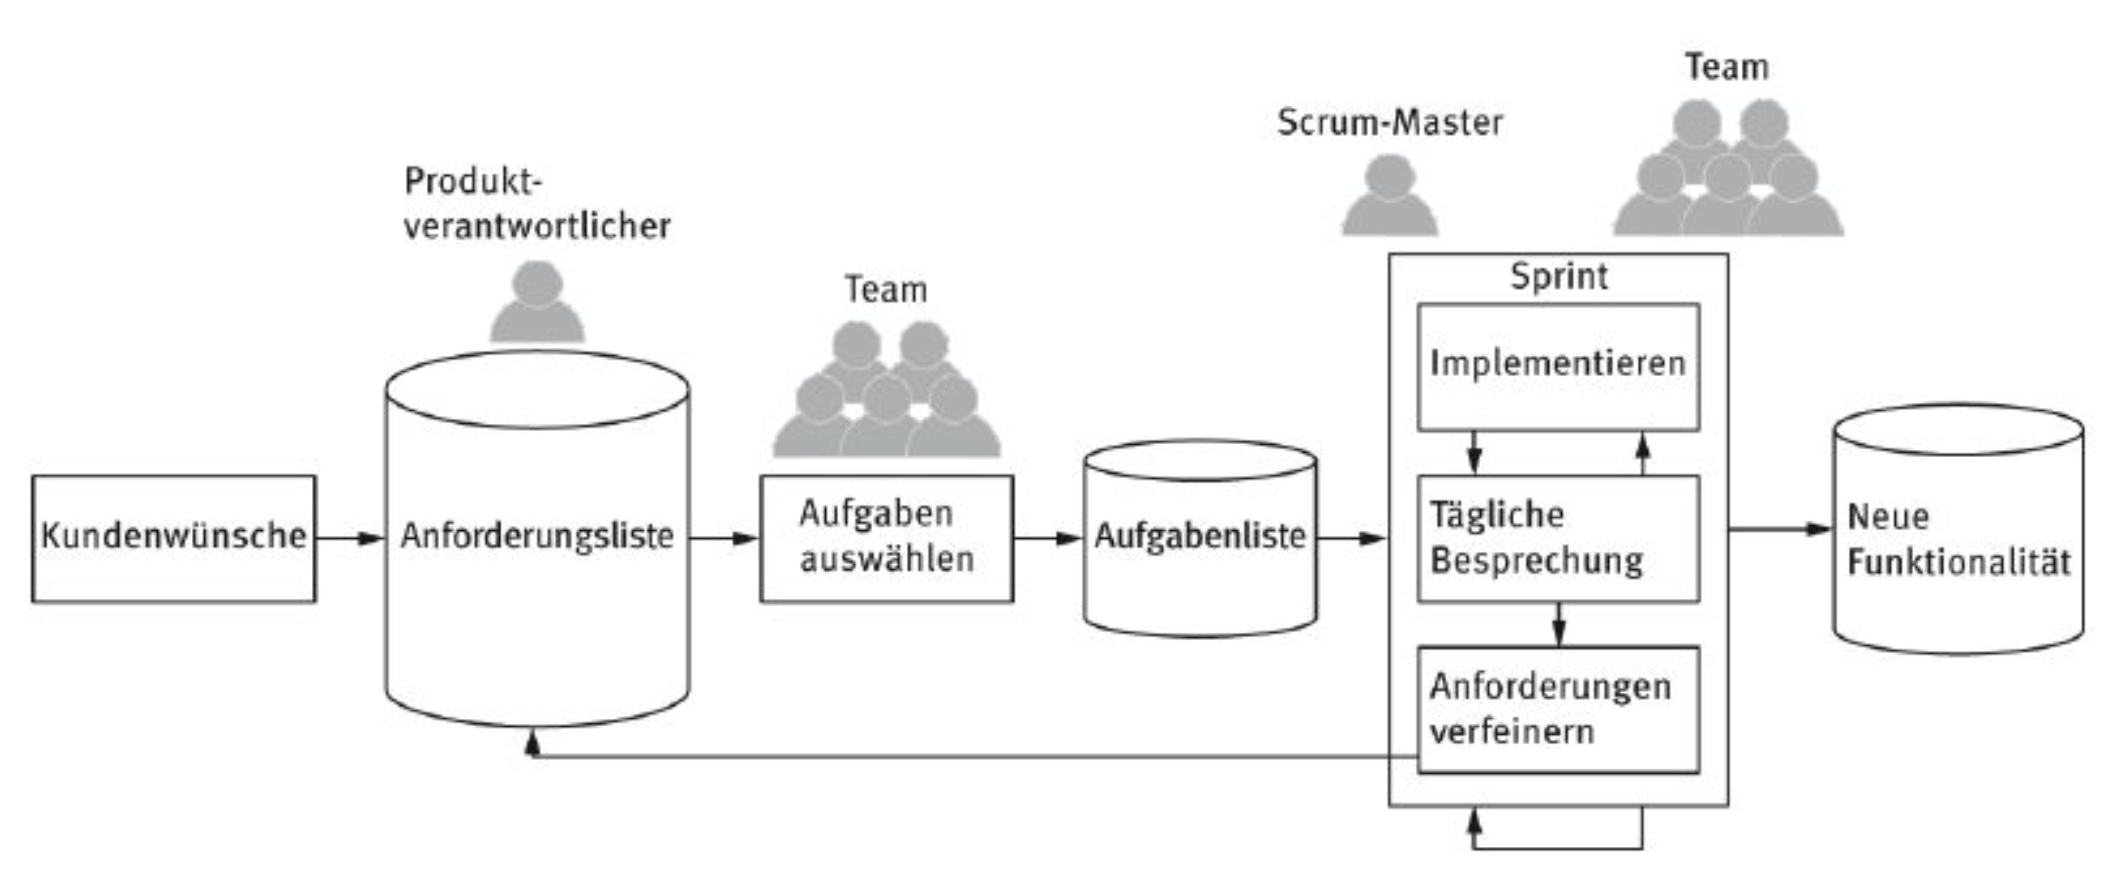
\includegraphics[width=0.8\textwidth]{assets/Scrum.png}
\end{figure}
